\documentclass[9pt]{beamer}
\usepackage[boldfont]{xeCJK}
\usepackage{mathtools}
\usepackage{amsmath, amssymb, amsthm}
\usepackage{mathpartir}
\usepackage{lstautogobble}
\usepackage{syntax}
\usepackage{listings}
\usepackage{xcolor}
\usepackage{indentfirst}
\usepackage{tikz}
\usepackage{shorttoc}

\usetheme{Copenhagen}
\newcommand{\xto}{\xrightarrow}
\let\emptyset\varnothing

\setmainfont[Scale=1.08]{Charter}
\setCJKmainfont[Scale=1.15]{STSong}
\setCJKfamilyfont{kai}{Kaiti SC}

\newfontfamily\listingsfont{PT Mono}

\linespread{1.3}
\lstset{
        basicstyle=\listingsfont\linespread{0.1},
        keywordstyle=\bfseries\color{blue},
        commentstyle=\itshape\color{gray},
        numberstyle=\color{black}
}
\lstdefinelanguage{Ocaml}{morekeywords={fun, let, in,if,then,else}}

\title{面向Hindley-Milner类型系统的控制流分析算法}
\author[Xiangyu Luo]{罗翔宇}
\institute[sist]{北京大学\\信息科学技术学院}

\begin{document}
    \begin{frame}
        \titlepage
    \end{frame}
    
    \section{背景介绍}
    \begin{frame}{控制流分析}
        \begin{itemize}
        		\item 当今程序的静态分析在软件工程领域扮演了越来越重要的角色,代码漏洞检测、代码优化等都离不开程序静态分析的结果
		\vspace{0.8em}
		\item 而控制流分析是静态分析一个最基础的环节,有了控制流分析的结果,就可以做数据流分析、程序切片等静态分析
        \end{itemize}
    \end{frame}
    
\begin{frame}[fragile]{函数式语言的控制流分析}
    	\begin{itemize}
		\item 函数式语言中,一个表达式的控制流分析结果即为该表达式最终求值的可能结果的集合。
        \begin{lstlisting}[language=Ocaml]
	let f = fun x -> if x then False else True
	in f True
        \end{lstlisting}
        \end{itemize}
\end{frame}
    
\begin{frame}{基于类型系统的控制流分析}
	\begin{itemize}
		\item 基于类型系统的控制流分析相比于基于抽象解释的控制流分析,有着效率高、模块化强、求值顺序无关等特点。
		\vspace{0.8em}
		\item Mossin 提出了基于类型系统的控制流分析算法,但是只能应用于简单的$\lambda$演算类型系统。 我们尝试将其扩展到Hindley-Milner类型系统上。
	\end{itemize}
\end{frame}

\begin{frame}{背景介绍 - Hindley-Milner 类型系统}
	目前Haskell, Ocaml等主流函数式编程语言的类型系统都基于Hindley-Milner类型系统。相比于其它类型系统,它有以下两个特点:
	\vspace{1.5em}
	\begin{itemize}
		\item 函数参数类型免于声明,可以通过类型重建重建出
		\item let语句绑定的变量都具有多态性
	\end{itemize}
	\vspace{1.5em}
	这两个特点为开发人员编写程序提供了极大的便利,但是也为我们的控制流分析带来了挑战。
\end{frame}

\section{算法框架}

\begin{frame}[fragile]{背景介绍 - HM类型系统的参数重建}
	\begin{itemize}
		\item HM类型系统中,所有的函数参数均可以不用声明类型。
		\vspace{0.3em}
		\item 我们要为每一个函数参数分配一个类型变量,然后在根据参数的使用将对应的参数变量添加进一个类型约束集合,最终解类型约束集合得到每个类型变量所代表的真实类型。
		\vspace{0.3em}
		\item 代码示例:\begin{lstlisting}[language=Ocaml, escapeinside={`}{`}]
(fun`$^{\ell_1}$` x -> if`$^{\ell_2}$` x`$^{\ell_3}$` then True`$^{\ell_4}$` else False`$^{\ell_5}$`) True`$^{\ell_6}$`
		\end{lstlisting}
		\vspace{0.2em}
		\item 这里我们有类型约束:$\{X = Bool,\ X\to Y = Bool\to Y,\ Y = Bool\}$
	\end{itemize}
\end{frame}

\begin{frame}[fragile]{背景介绍 - Mossin控制流分析算法}
	\begin{itemize}
		\item Mossin的算法基于扩展的带有流属性的类型系统。
		\vspace{0.5em}
		\item 所谓流属性类型即为每一个原始类型都绑定一个标号集合,表明拥有该类型的表达式,最终可能的求值结果的标号集合。
		\item 带标号的程序示例:
		\begin{lstlisting}[language=Ocaml, escapeinside={`}{`}]
(fun`$^{\ell_1}$` x -> if`$^{\ell_2}$` x`$^{\ell_3}$` then True`$^{\ell_4}$` else False`$^{\ell_5}$`) True`$^{\ell_6}$`
		\end{lstlisting}
		\item 这里使用我们的算法可以推导出前面函数的类型为$Bool^{\ \ell_6}\xrightarrow{\ell_1}Bool^{\ \{\ell_4, \ell_5\}}$, 整个表达式的类型为$Bool^{\ \{\ell_4, \ell_5\}}$
	\end{itemize}
	\vspace{0.2em}
	由于所有子表达式的标号都是互不相同的,故一旦完成了类型推导,就可以根据表达类型得到其控制流分析的结果。
\end{frame}


\begin{frame}[fragile]{流属性变量及流属性变量约束集合}
	\begin{itemize}
		\item 我们需要一个流属性变量来代指任何类型的流属性。维护类型约束集合的同时也要维护一个流属性约束集合,最终求解流属性约束集合。
		\vspace{0.3em}
		\item 代码示例:
		\vspace{0.2em}
		\begin{lstlisting}[language=Ocaml, escapeinside={`}{`}]
(fun`$^{\ell_1}$` x -> if`$^{\ell_2}$` x`$^{\ell_3}$` then True`$^{\ell_4}$` else False`$^{\ell_5}$`) True`$^{\ell_6}$`
		\end{lstlisting}
		\vspace{0.3em}
		\item 我们这里有流属性约束集合:$\{\{\ell_6\}\subseteq\alpha,\ \{\ell_4, \ell_5\}\subseteq \beta\}$
	\end{itemize}
\end{frame}

\begin{frame}[fragile]{类型变量实例化}
	\begin{itemize}
		\item 一个问题是,我们不能简单地将类型变量直接实例化为类型
		\begin{lstlisting}[language=Ocaml,escapeinside={`}{`}]
			if True then fun`$^{\ \ell_1}$` x -> True`$^{\ \ell_3}$` else fun`$^{\ \ell_2}$` x -> False`$^{\ \ell_4}$`
		\end{lstlisting}
		\vspace{0.2em}
		\item 考虑如上代码,我们有类型约束集合$\{X^{\ \alpha} = Y^{\ \beta}\xrightarrow{\{\ell_1\}}Bool^{\{\ell_3\}}\}$和$\{X^{\ \alpha} = Z^{\ \gamma}\xrightarrow{\{\ell_2\}}Bool^{\{\ell_4\}}\}$。 子类型约束集合:$\{X^{\ \alpha} \succeq Y^{\ \beta}\xrightarrow{\{\ell_1\}}Bool^{\{\ell_3\}}\}$和$\{X^{\ \alpha} \succeq Z^{\ \gamma}\xrightarrow{\{\ell_2\}}Bool^{\{\ell_4\}}\}$
		\vspace{0.2em}
		\item 如果我们简单地把$X$替换,就会在子类型约束集合中导出矛盾。所以我们需要在替换时只替换类型,而把所有的流属性用新的流属性变量替代。
	\end{itemize}
\end{frame}

\begin{frame}[fragile]{挑战 - let多态绑定}
	\begin{itemize}
		\item 在Hindley-Milner类型系统中,处理let多态的方式为,先求出绑定的表达式的主类型T,以及记录当前表达式产生的类型约束集合S。
		\vspace{0.2em}
		\item 求解约束集合S,并将其解应用到当前环境和后续的分析过程中。
		\vspace{0.2em}
		\item 但是由于子类型约束集合不能部分求解, 所以我们需要将集合记录在类型中。
	\end{itemize}
\end{frame}

\begin{frame}[fragile]{解决方案 - 流属性类型模板}
	\begin{itemize}
		\item 考虑代码:
		\vspace{0.2em}
		\begin{lstlisting}[language=Ocaml,escapeinside={`}{`}]
			let f = `$\lambda$`x`$\alpha$`.`$\lambda$`y`$\beta$`. if True then x else y
			in (f 1, f True)
		\end{lstlisting}
		\vspace{0.3em}
		\item 这里我们推导出f的类型即为$\forall\alpha\ \beta.\{\alpha\subseteq\gamma,\ \beta\subseteq\gamma\}\Rightarrow\forall X\ Y.X^\alpha\to Y^\beta\to Z^\gamma$
	\end{itemize}
\end{frame}

\begin{frame}[fragile]{挑战 - 约束集合指数爆炸}
	\begin{itemize}
		\item 考虑如下程序
		\begin{lstlisting}[escapeinside={`}{`}, language=Ocaml]
	let x0 = e in
		let x1 = fun y -> if y then x0 else x0 in
			let x2 = fun z -> if z then x1 else x1 in
				...
		\end{lstlisting}
		\item 不妨设推导e时,产生了流属性约束集合$C_0$,接下来推导x1的绑定表达式时,其约束集合$C_1$中包含$C_0$的两个拷贝,而同理$C_2$中也包含$C_1$的两个拷贝
		\vspace{0.3em}
		\item 流属性约束集合的大小随着let的嵌套层数而指数爆炸
	\end{itemize}
\end{frame}

\begin{frame}[fragile]{解决方案 - 合并冗余约束}
	可以发现有一些约束是多余的,可以将其合并为一条约束:
	\vspace{0.5em}
	\begin{itemize}
				\item 如果约束集合中存在$\{\ell_1\subseteq \alpha, \ell_2\subseteq \alpha\}$的约束,可以将其合并为$\{\ell_1\cup\ell_2 \subseteq \alpha\}$. 
		\vspace{0.3em}
		\item 如果约束集合中存在$\{\ell_1 \subseteq \alpha, \ell_2 \subseteq \alpha, \alpha\subseteq \beta\}$,且$\alpha$在表达式无自由出现,那么可以将其合并为$\{\ell_1\cup\ell_2\subseteq\beta\}$
	\end{itemize}
	\vspace{0.5em}
	可以发现合并过约束之后,流属性约束集合中变量的个数最多只有$O(n)$个,故最多有$O(n^2)$条约束
\end{frame}

\begin{frame}[fragile]{求解流属性约束}
	\begin{itemize}
		\item 我们可以将流属性约束转化为一个图来进行求解。
		\vspace{0.3em}
		\item 如果有约束$\{\alpha\preceq\beta\}$, 则在其之间连接一条有向边
		\vspace{0.3em}
		\item 可以发现一个变量所代表的流属性集合,即是它在此图中可以到达的所有顶点的流属性集合的并集
	\end{itemize}
\end{frame}

\begin{frame}[fragile]{求解流属性约束}
	\begin{itemize}
		\item 我们先考虑这个图没有环的情况,此时该图可以拓扑排序,然后按照拓扑排序的结果使用动态规划求解即可。
		\vspace{0.5em}
		\begin{center}
	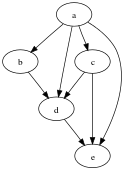
\includegraphics[width=1.8cm]{DAG.png}
	\end{center}
		\vspace{0.2em}
		\item 如果有环的话,我们可以使用Tarjan算法收缩图的极大强连通分量,然后在收缩过的新图上使用有向无环图的算法求解,再根据原图顶点和强连通分量之间的对应关系,计算出原图顶点的流属性集合。
	\end{itemize}
\end{frame}

\section{实验测试}

\begin{frame}[fragile]{实验目标}
	我们的实验目标主要有以下两点:
	\vspace{0.5em}
	\begin{itemize}
		\item 测试算法的运行效率
		\vspace{0.3em}
		\item 测试算法的正确性以及准确率
	\end{itemize}
\end{frame}

\begin{frame}[fragile]{实验设计}
	为了验证以上目标,我们设计了如下两个测试文件:
	\vspace{0.5em}
	\begin{itemize}
		\item medium.hs文件由20层嵌套的let语句组成,为了测试let嵌套时的运行效率,防止约束集合指数爆炸。
		\vspace{0.3em}
		\item 而large.hs文件由107行haskell代码构成,其中包含ski组合子、基于$\lambda$演算定义的邱奇数、基于$\lambda$演算定义的元组函数、列表函数等各种较为复杂的函数。由于目前运行在Haskell语言上的模块化控制流分析算法只有CHA,故我们的准确度和CHA算法作比较。
	\end{itemize}
	\vspace{0.2em}
	其中medium.hs用于验证let嵌套的优化,large.hs用于验证算法效率和准确度。
\end{frame}

\begin{frame}[fragile]{实验结果}
	\begin{itemize}
		\item medium.hs文件在0.098秒内即可运行出解,如果去掉项目中针对let嵌套的优化,则会在运行大约20秒之后因为占用内存过大而崩溃退出。 这说明我们针对let嵌套的优化有效。
		\vspace{0.2em}
		\item large.hs文件在1.688秒内即可运行出解,说明我们算法效率良好。
		\vspace{0.2em}
		\item 对于large.hs文件,我们的控制流算法共分析出了1319处目标函数调用的结果,而CHA则分析出有1996处目标函数调用结果,相当于将CHA的准确度提升了$34\%$。
		\vspace{0.2em}
		\item 注意到CHA随着程序代码量的上升,准确度会进一步下降,故我们的算法在分析更大规模的程序时,相比于CHA的准确度会进一步提高。
	\end{itemize}
\end{frame}

\begin{frame}[fragile]{提问环节}
	\begin{itemize}
		\item Thank you 
		\vspace{1em}
		\item Q\&A
	\end{itemize}
\end{frame}

\end{document}
